% ---- ETD Document Class and Useful Packages ---- %
\documentclass{ucetd}
\usepackage{subfigure,epsfig,amsfonts}
\usepackage{natbib}
\usepackage{amsmath}
\usepackage{amssymb}
\usepackage{amsthm}
\usepackage[toc,page]{appendix}
\usepackage[labelfont=bf]{caption}
\usepackage{rotating}
\usepackage[dvipsnames]{xcolor}
\usepackage{url}
\usepackage{bm}
\usepackage{bbm}

%% Use these commands to set biographic information for the title page:
\title{Visualizing nucleosome cluster dynamics with dense single molecule localization microscopy}
\author{Clayton W. Seitz}
\department{Department of Physics}
\division{Physical Sciences}
\degree{Doctor of Philosophy}
\date{Spring 20XX}

%% Use these commands to set a dedication and epigraph text

\epigraph{Epigraph}



\begin{document}
%% Basic setup commands
% If you don't want a title page comment out the next line and uncomment the line after it:
\maketitle
%\omittitle

% These lines can be commented out to disable the copyright/dedication/epigraph pages
\makecopyright
%\makededication


%% Make the various tables of contents
\tableofcontents
%\listoffigures
%\listoftables

%\acknowledgments
% Enter Acknowledgements here

\abstract

Single-molecule localization-based super-resolution microscopy techniques, such as direct stochastic optical reconstruction microscopy (dSTORM), can be used to produce a pointillist representation of nucleosome organization at diffraction-unlimited precision. Direct STORM approaches leverage the deactivation of fluorescent tags, followed by spontaneous or photoinduced reactivation, to achieve super-resolution reconstructions of nuclear proteins and nucleic acids. This basic principle remains one of the method's primary limitations - standard analysis algorithms require tight control of activation and reactivation to maintain sparse emitters, presenting a tradeoff between imaging speed and labeling density. Here, we present a dSTORM strategy for fast reconstruction of nucleosome organization in living cells by complementing high duty-cycle blinking of rhodamine-derived dyes with a novel localization algorithm based on deep generative modeling. Previous approaches to breaking the time resolution barrier in SMLM learn prior information about cellular structures using generative models and predict super-resolution images based on sparse localizations, or interpolate and transform dense images into a localization map. However, cellular structures such as chromatin are dynamic and intrinsically heterogeneous; therefore, structures cannot necessarily be known apriori. Furthermore, localization maps are parametric and non-probabilistic, making them highly application specific, and difficult to use. We propose an alternative method based on directly modeling the distribution of high resolution images conditioned on a low resolution image. By performing high density localization, we can directly visualize 1,6 Hexanediol induced chromatin reorganization over minute time scales.


\clearpage

\mainmatter

\chapter{}

\section{Introduction}

\subsection{Photoswitchable rhodamine derivatives for super-resolution microscopy}


\begin{figure}
\begin{center}
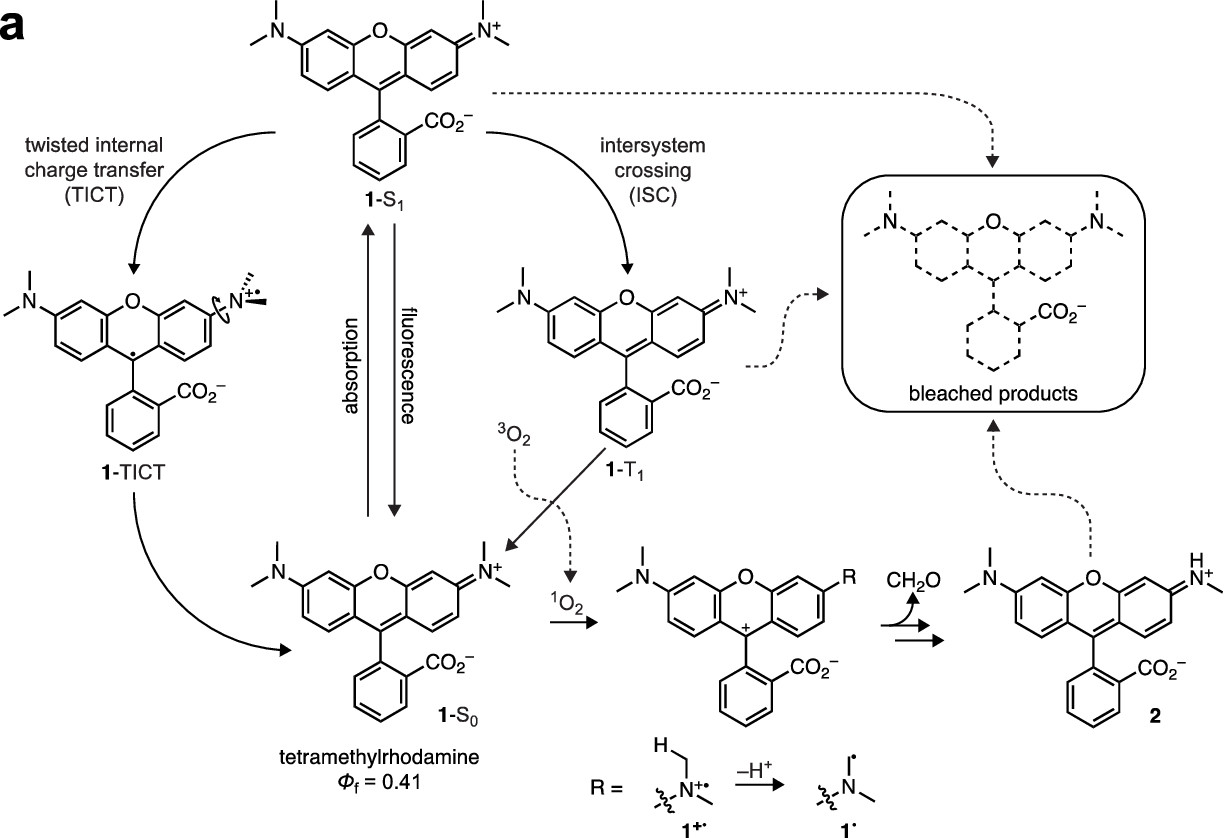
\includegraphics[width=14cm]{Rhodamines.png}
\end{center}
\end{figure}

Single molecule localization microscopy (SMLM) relies on the temporal resolution of fluorophores in the sample whose spatially overlapping point spread functions would otherwise render them unresolvable at the detector. SMLM techniques remain desirable for super-resolution imaging of many cellular structures, due to their cost-effective implementation and photon-count limited resolution (Schermelleh 2019). Common strategies for the temporal separation of molecules involve intramolecular rearrangements to switch from dark to fluorescent states or the exploitation of non-emitting molecular radicals. For live cell super-resolution of chromatin nanodomains, the HaloTag fusion protein and its associated JF549-HaloTag and JF646-HaloTag ligands have surfaced as indispensable tools (Grimm 2015). H2B is a suitable choice, since it is one of the histones with fewer tail modifications and functional variants with known function (Kamakaka 2005). Reduced rhodamine derivates like JF549 and JF646 can be quenched by oxidative processes or form dark radical species, which absorb strongly around 400 nm, a property that can be exploited to drive the fluorophore back to its ground state. Long dark state lifetimes are commonly used in STORM imaging, while quenching results in higher duty cycle and increased rates of photobleaching due to irreversible oxidative damage of important functional groups. Nevertheless, high duty cycle SMLM can greatly reduce acquisition times and increase labeling density while permitting the recording of some dynamic processes (Speiser 2021).  

Super-resolved nucleosome organization has been studied extensively in various epigenomic states to reveal segregated nanoclusters, dispersed nanodomains, and compact large aggregates  8–10 . Nucleosomes assemble into heterogeneous clusters of variable sizes, interspersed with nucleosome-depleted regions (Ricci 2015). Histone modifications regulate the packaging of nucleosomes into a higher-order chromatin structure to influence the accessibility of genomic DNA to transcription machinery. Higher-order chromatin structure is implicated in a number of cellular processes including gene regulation (Hnisz 2017; Sabari 2018; Boija 2018), DNA damage and repair (Locatelli 2022), as well as cell differentiation and immune activation (Lin 2022). However, identification of key determinants of nucleosome organization at super-resolution remains limited by a lack of live cell and high frame-rate SMLM techniques. Direct visualization of dynamic nucleosome organization over a time scale of hours could provide new insights into the role of higher order chromatin organization in a variety of cellular functions.  

Here, we provide an approach to fast reconstruction of nucleosome organization in living cells. Previous approaches to live cell imaging of chromatin nanodomains only provide ensemble snapshots of chromatin structure due to slow acquisition times (Nozaki 2017). By leveraging the long dark state lifetime of JF646 at moderate laser power, we reconstruct a map of H2B organization in living Hela cells, without sacrificing considerable resolution. Resolution in SMLM is more nuanced and scales with the signal to noise ratio (SNR) and the geometry of the underlying biological structure. Therefore, we develop an image formation model which accounts for sCMOS noise characteristics, molecular density as measured with Ripley’s K-function (Ripley 1977), and a two-state photoswitching model. The sCMOS camera architecture results in every pixel having a unique noise characteristic, and the noise variances of individual pixels can reach thousands of analog-to-digital units squared (Huang 2013). This localization problem is exacerbated in dense scenarios where localization precision and detection accuracy diminish for high duty cycle photoswitching, resulting in significant deviations from the Cramer-Rao lower bound (Speiser 2021). We circumvent these challenges by combining high duty cycle dSTORM with a convolutional neural network (CNN) architecture for fast and accurate single molecule localization (Speiser 2021, Nehme 2020). 

To visualize dynamics of nucleosome organization in interphase nuclei, we recorded dSTORM time-series using oblique illumination microscopy to illuminate a thin area within a single nucleus (Tokunga 2008; Nozaki 2017). By leveraging high duty cycle SMLM and model-based localization algorithms, we efficiently utilize the photon budget and capture super-resolution movies of HaloTag-H2B over long time scales. Our approach complements the short lifetime non-fluorescent state of a HaloTag ligand in a reducing environment with a localization algorithm trained on simulated dense SMLM time-series (iterative Richardson-Lucy deconvolution with the point spread function and maximum likelihood fitting). The method is extended further by two-color labeling to reveal the respective partitions of fast and slow-diffusing H2B in relation to the structure of chromatin nanodomains.  

We demonstrate our approach by characterizing microscale nucleosome organization and dynamics in response to external cues e.g., immune signaling. We use density estimation to predict the generating distribution for pointillist H2B data, which allows us to simultaneously define clusters in the dataset, observe cluster dynamics in time, and compensate for low sample counts. 


Single molecule localization microscopy (SMLM) is a type of super-resolution microscopy that allows the imaging of fluorescently-labeled molecules with high precision, well beyond the diffraction limit of light. SMLM techniques such as direct stochastic optical reconstruction microscopy (dSTORM), photoactivated localization microscopy (PALM), and related methods rely on the precise localization of single molecules by resolving them in time rather than space. By combining the precise localization of many individual molecules, SMLM can generate images with resolution down to a few nanometers. SMLM has been used in a variety of applications, including the imaging of subcellular structures such as synapses, mitochondria, and cytoskeletal elements, as well as the study of protein-protein interactions, molecular dynamics, and other biological processes at the nanoscale level.

Despite its successs and gaining popularity, the basic principle of SMLM is one of its primary limitations: the need for sparse activation leads to long acquisition times and expensive autofocusing equipment to actively correct for sample drift. This results in low throughput, poor time resolution when imaging dynamic processes, low labeling densities and a reduced choice of fluorophores. In addition, the need for sparse activation requires laborious optimization of dSTORM buffers containing oxygen scavenging systems and/or oxygen purging techniques. In response to these problems, a host software tools for SMLM have emerged, which permit the acquisition of emitters at higher densities. (Speiser 2021). In the multi-emitter setting, PSFs are no longer well-separated but may overlap, adding additional 1uncertainty into the localization process. Existing algorithms have explicitly modeled the point spread function as a mixture of single molecule PSFs or have utilized deep learning-based tools to estimate the parameters of each PSF embedded in the mixture.  

Due to overlap, conventional detection strategies may undercount the emitters in a local neighborhood in some frames, localization uncertainty can increase for overlapping emitters, and some localizations may be missed entirely. These complications make conventional detection strategies inappropriate for reconstruction of super-resolution images from time-series. Perhaps most importantly, overlapping emitters can result in additional localization uncertainty, rendering discernment between the arrival of a new particle and a poorly localized existing one difficult. This issue poses a major bottleneck to super-resolution imaging acqusitions. Additional uncertainty can be partially alleviated by using pairwise or higher-order temporal correlations within a pixel neighborhood to deconvolve individual emitters. A similar idea is employed in super-resolution optical fluctuation imaging (SOFI) - a post-processing technique that uses image cumulants to deconvolve emitters. 

\subsection{Efficient computation of the Cramer-Rao lower bound}


\begin{figure}
\begin{center}
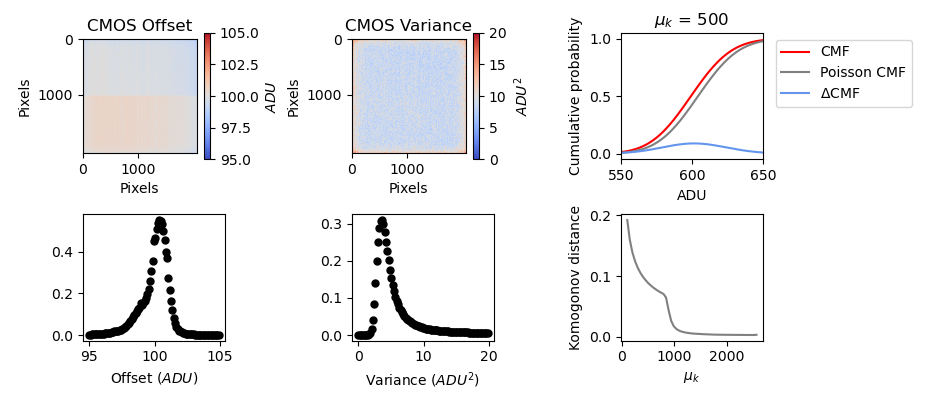
\includegraphics[width=16cm]{Noise.png}
\end{center}
\end{figure}


We are now prepared to write the shot-noise limited signal, which is a vector with units of phototelectrons

\begin{equation}
\vec{S} = \left[\mathrm{Poisson}(\mu_{1}), \mathrm{Poisson}(\mu_{2}), ..., \mathrm{Poisson}(\mu_{N})\right]
\end{equation}


However this noise model is incomplete, because detectors often suffer from dark noise, which may refer to readout noise or dark current, and contributes to a nonzero signal even in the absence of incident light. Dark current is due to statistical fluctuations in the photoelectron count due to thermal fluctuations. Readout noise is introduced by the amplifier circuit during the coversion of photoelectron charge to a voltage. Here, we use the Hamamatsu ORCA v3 CMOS camera, which is air cooled to -10C and has very low dark current - around 0.06 electrons/pixel/second - and can therefore be safely ignored for exposure times on the order of milliseconds. Readout noise has been often neglected in localization algorithms because its presence in EMCCD cameras is small enough that it can be ignored within the tolerances of the localization precision. In the case of sCMOS cameras, however, the readout noise of each pixel is significantly higher and, in addition, every pixel has its own noise and gain characteristic sometimes with dramatic pixel-to-pixel variations.

It is important to note that we cannot measure the contribution by readout noise before amplification and therefore it must be expressed in units of $\mathrm{ADU}$. This is in contrast to $\vec{S}$, which can be expressed in units of photoelectrons, because these statistical fluctuations can be predicted to be Poisson by quantum mechanics. Furthermore, the number of photoelectrons $S_{k}$ is  multiplied by a gain factor $g_{k}$ which has units of $[\mathrm{ADU}/e^{-}]$, which generally must be measured for each pixel. Here, we will always assume that readout noise per pixel $\xi_{k}$ is Gaussian with some pixel-specific offset $o_{k}$ and variance $\sigma_{k}^{2}$. We will also assume that gain factors and pixel noise characteristics are constants and do not scale with the signal level $S_{k}$. Therefore our measurement, in units of ADU, is: 

\begin{equation}
\vec{H} = \vec{S} + \vec{\xi}
\end{equation}

What we are after is the joint distribution $P(\vec{H})$. A fundamental result in probability theory is that the distribution of $H_{k}$ is the convolution of the distributions of $S_{k}$ and $\xi_{k}$,

\begin{align}
P(H_{k}|\theta) &= P(S_{k})\circledast P(\xi_{k})\\
&= A\sum_{q=0}^{\infty} \frac{1}{q!}e^{-\mu_{k}}\mu_{k}^{q}\frac{1}{\sqrt{2\pi}\sigma_{k}}e^{-\frac{(H_{k}-g_{k}q-o_{k})}{2\sigma_{k}^{2}}}
\end{align}

where $P(\xi_{k}) = \mathcal{N}(o_{k},\sigma_{k}^{2})$ and $P(S_{k}) = \mathrm{Poisson}(g_{k}\mu_{k})$. In practice, this expression is difficult to work with, so we look for an approximation. Notice that 

\begin{align*}
\xi_{k} - o_{k} + \sigma_{k}^{2} \sim \mathcal{N}(\sigma_{k}^{2},\sigma_{k}^{2}) \approx \mathrm{Poisson}(\sigma_{k}^{2})
\end{align*}

Since $H_{k} = S_{k} + \xi_{k}$, we transform $H_{k}' = H_{k} - o_{k} + \sigma_{k}^{2}$, which is distributed according to 

\begin{align*}
H_{k}' \sim \mathrm{Poisson}(\mu_{k}')
\end{align*}

where $\mu_{k}' = g_{k}\mu_{k} + \sigma_{k}^{2}$. This result can be seen from the fact the the convolution of two Poisson distributions is also Poisson.

\subsubsection{Integrated isotropic Gaussian point spread function}

Due to diffraction, any point emitter, such as a single fluorescent molecule, will be registered as a diffraction limited spot. It is common to describe the point spread function as a two-dimensional isotropic Gaussian:

\begin{equation*}
\mathrm{G}(x,y) = \frac{1}{2\pi\sigma^{2}}e^{-\frac{(x-x_{0})^{2}+(y-y_{0})^{2}}{2\sigma^{2}}}
\end{equation*}

Modern cameras used in light microscopy, such as scientific complementary metal oxide semiconductor (sCMOS) cameras, are powered by the photoelectric effect. Electrons within each pixel, called photoelectrons, absorb enough energy from incoming photons to be promoted to the conduction band to give electrical current which can be detected. Integration of photoelectrons during the exposure time results in a monochrome image captured by a camera. The image of a single point particle, such as a fluorescent molecule, can be thought of as two-dimensional histogram of photon arrivals and a discretized form of the classical intensity profile $\mathrm{G}(x,y)$. The value at a pixel approaches an integral of this density over the pixel:

\begin{equation}
\mu_{k} = i_{0}\lambda_{k} = i_{0}\int_{\mathrm{pixel}} G(x,y)dxdy
\end{equation}

Let $(x_{k},y_{k})$ be the center of pixel $k$. If a fluorescent molecule is located at $(x_{0},y_{0})$, the probability of a photon arriving at pixel $k$ per unit time reads

\begin{equation*}
\lambda_{k} = \int_{x_{k}-\frac{1}{2}}^{x_{k}+\frac{1}{2}}G(x-x_{0})dx \int_{y_{k}-\frac{1}{2}}^{y_{k}+\frac{1}{2}} G(y-y_{0})dy
\end{equation*}

\vspace{0.2in}
where $i_{0} = g_{k}\eta N_{0}\Delta$. The parameter $\eta$ is the quantum efficiency and $\Delta$ is the exposure time. $N_{0}$ represents the number of photons emitted per unit time, which may be itself a Poisson random variable; however, this is inconsequential since it is a fixed value for a single image of a fluorescent molecule. We can then express the Gaussian integrals over a pixel by making use of the following property of the error function

\begin{equation*}
\frac{1}{\sqrt{2\pi}\sigma}\int_{a}^{b} e^{\frac{-(x-\mu)^{2}}{2\sigma^{2}}} = \frac{1}{2}\left(\mathrm{erf}\left(\frac{b-\mu}{\sqrt{2}\sigma}\right) -\mathrm{erf}\left(\frac{a-\mu}{\sqrt{2}\sigma}\right)\right)
\end{equation*}

This gives a convenient expression for the fraction of photons which arrive at a pixel $k$

\begin{align*}
\lambda_{k}(x) &= \frac{1}{2}\left(\mathrm{erf}\left(\frac{x_{k}+\frac{1}{2}-x_{0}}{\sqrt{2}\sigma}\right) -\mathrm{erf}\left(\frac{x_{k}-\frac{1}{2}-x_{0}}{\sqrt{2}\sigma}\right)\right)\\
\lambda_{k}(y) &= \frac{1}{2}\left(\mathrm{erf}\left(\frac{y_{k}+\frac{1}{2}-y_{0}}{\sqrt{2}\sigma}\right) -\mathrm{erf}\left(\frac{y_{k}-\frac{1}{2}-y_{0}}{\sqrt{2}\sigma}\right)\right)
\end{align*}

\subsubsection{Integrated astigmatic Gaussian point spread function}

In 2D SMLM simulations, a 2D PSF  model  with  a z-dependent  isotropic  width $\sigma$ can  be  used. For 3D, we could use that the isotropic Gaussian point spread function has a FWHM $\sigma$ which is dependent on the axial coordinate. However, it can be shown that the error around the focus is very large and negative and positive defocus cannot be distinguished given the symmetric dependence in $z$.  Therefore, for 3D SMLM, a cost-effective approach is to introduce astigmatism into the detection path using a weak ($f\approx 10\mathrm{m}$) cylindrical lens. This gives an anisotropic Gaussian point spread function which is elongated perpendicular to the optical axis, depending on the axial ($z$) position of the fluorescent emitter. A fairly simple model for $\sigma_{x}(z_{0})$ and $\sigma_{y}(z_{0})$ upon defocus of a fluorescent molecule might be

\begin{equation*}
\sigma_{x}(z_{0}) = \sigma_{0} + \alpha(z_{0}+z_{min})^{2}\;\;\;\; \sigma_{y}(z_{0}) = \sigma_{0} + \beta(z_{0}-z_{min})^{2}
\end{equation*}

with the following continuous density over the pixel array

\begin{equation}
\mathrm{G}(x,y) = \frac{1}{2\pi\sigma_{x}(z)\sigma_{y}(z)}e^{-\frac{(x-x_{0})^{2}}{2\sigma_{x}(z_{0})^{2}}+\frac{(y-y_{0})^{2}}{2\sigma_{y}(z_{0})^{2}}}
\end{equation}


\subsubsection{Localization microscopy as frequentist inference}

According to our image formation, molecules really do have an exact location in space. In pratice, this is only an approximation since molecules diffuse at physiological temperatures, and our exposure time would need to tend to zero for this to be exactly true. If we suppose that we can collect a sufficient amount of photons in a short enough time, the physical nature of the system suggests a frequentist inference procedure for localization. A natural choice is maximum likelihood estimation. 

\begin{equation*}
\theta_{\mathrm{MLE}} = \underset{\theta}{\mathrm{argmax}}\prod_{k}P(H_{k}|\theta)= \underset{\theta}{\mathrm{argmin}}-\sum_{k}\log P(H_{k}|\theta)
\end{equation*}

Under the Poisson approximation, the model negative log-likelihood is

\begin{align}
\ell(\vec{H}|\theta) &= -\log \prod_{k} \frac{e^{-\left(\mu_{k}'\right)}\left(\mu_{k}'\right)^{n_{k}}}{n_{k}!}\\
&= \sum_{k}  \log n_{k}! + \mu_{k}' - n_{k}\log\left(\mu_{k}'\right)
\end{align}

When the log-likelihood is easy to compute, as it is under this approximation, we may ask: how much information does the data actually carry about parameters of our model? If the likelihood of the dataset is roughly constant for any parameter set we choose, we might expect our model cannot explain our observations. In other words, the data does not appear to carry much information about the parameters. After all, our posterior is being shaped in part by this likelihood. On the other hand, if $\ell$ has a number of bumps or inflection points, then we expect that maybe some parameter sets make our observed data more likely. The ``bumpiness" of the likelihood surface is called the Fisher information - a fundamental metric in information geometry. 

n order to calculate uncertainties in the molecular coordinates, in can be convenient to switch to the Bayesian point of view, where we know have to write the full posterior distribution, specifying a prior.


\section{Deep generative modeling with non-equilibrium thermodynamics}

\begin{figure}
\begin{center}
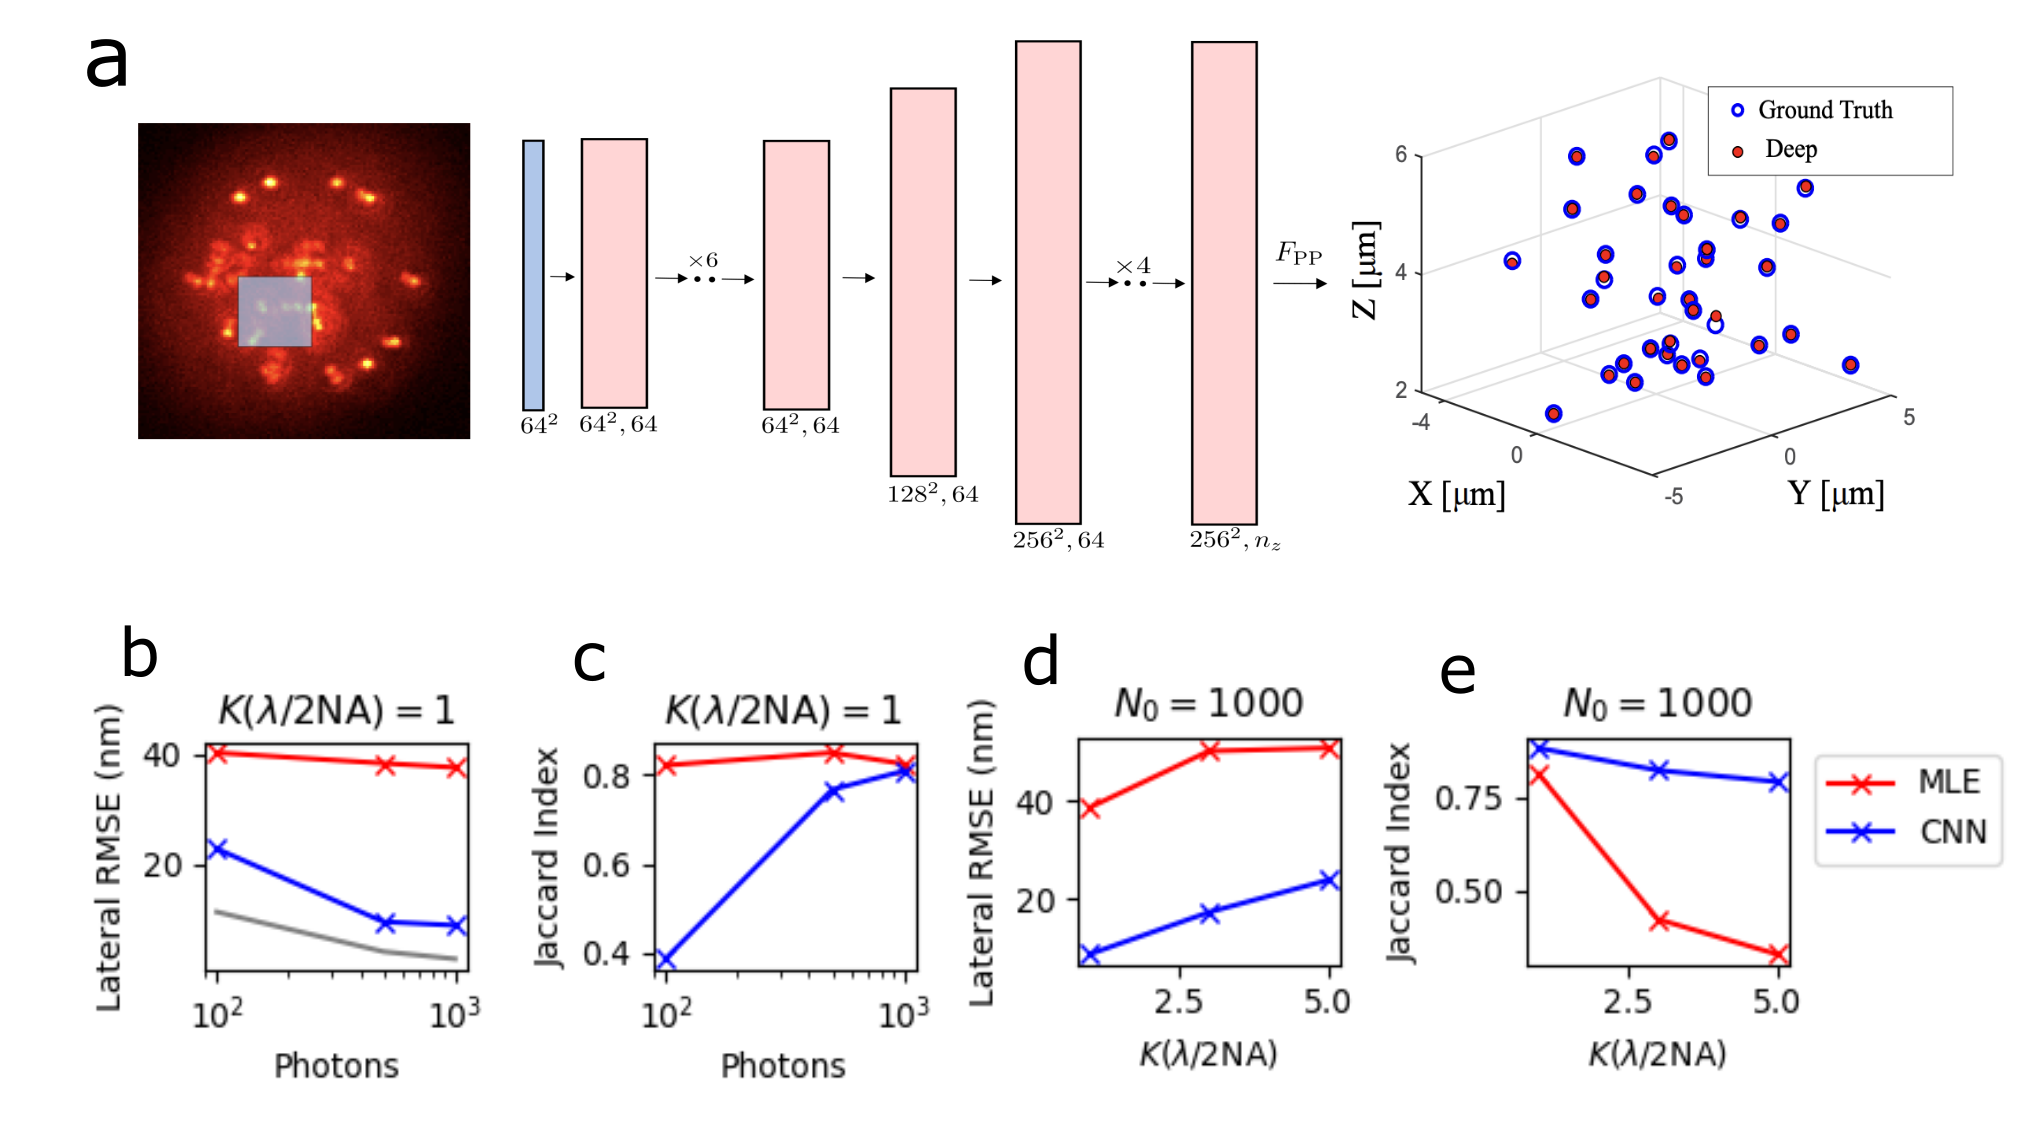
\includegraphics[width=16cm]{PSF2D.png}
\end{center}
\end{figure}

\begin{figure}
\begin{center}
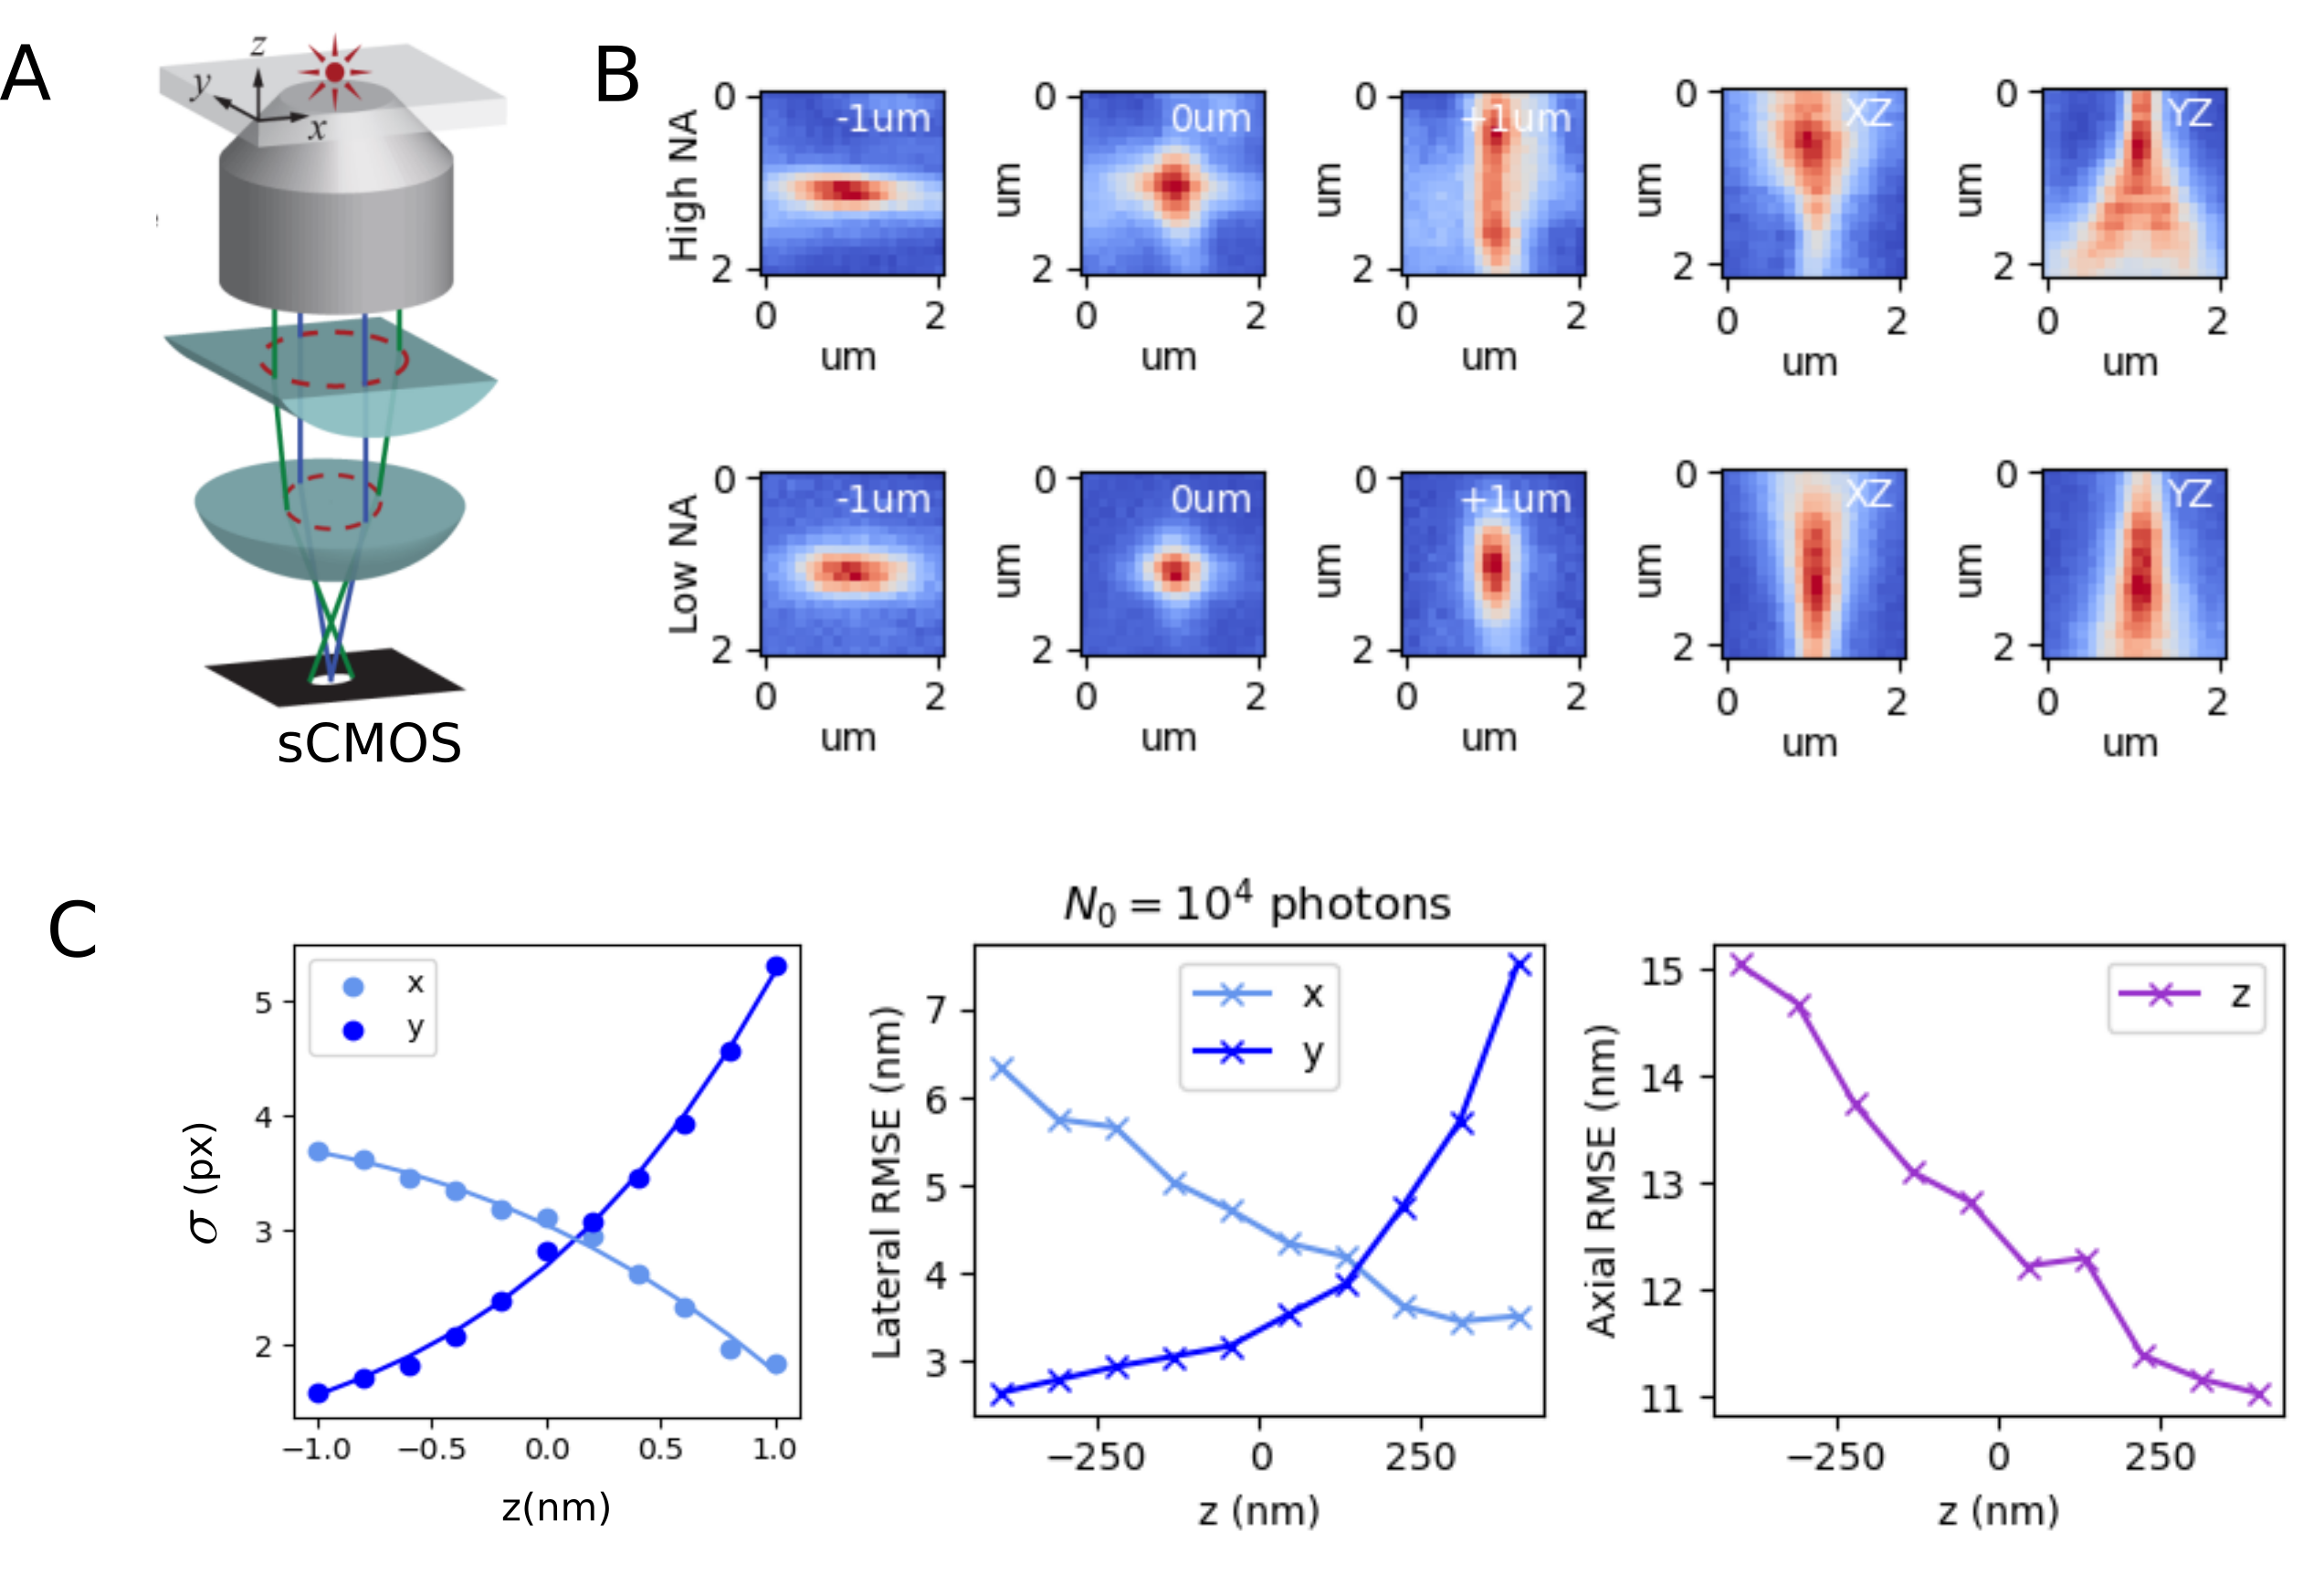
\includegraphics[width=16cm]{Astigmatism.png}
\end{center}
\end{figure}

\section{Visualizing nucleosome cluster dynamics in BRD4 condensates}

\begin{figure}
\begin{center}
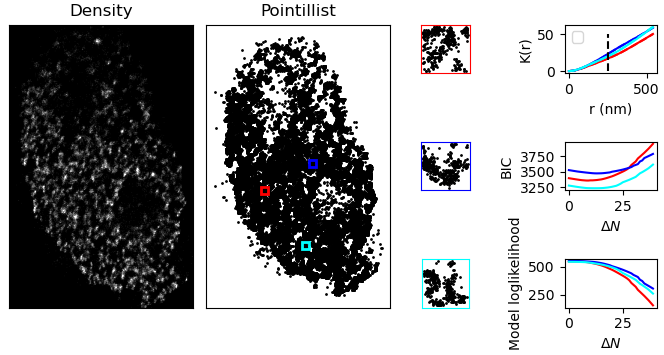
\includegraphics[width=16cm]{Cluster.png}
\end{center}
\end{figure}


\end{document}


